\documentclass[aspectratio=169,11pt,svgnames]{beamer}

\usepackage[czech]{babel}
\usepackage[czech=quotes]{csquotes}
\usepackage{graphicx}
\usepackage{enumitem}
\usepackage{amsmath}
\usepackage{mathtools}
\usepackage{float}
\usepackage{tikz}
\usepackage{caption}
\usepackage{subcaption}

% Flowchart stuff
\usetikzlibrary{shapes.geometric, arrows.meta, calc, positioning}
\tikzstyle{startstop} = [rectangle, rounded corners, minimum width=3cm, minimum
height=1cm,text centered, draw=black, fill=Red!30]
\tikzstyle{io} = [trapezium, trapezium left angle=70, trapezium right angle=110,
minimum width=3cm, minimum height=1cm, text centered, draw=black, fill=Blue!30]
\tikzstyle{process} = [rectangle, minimum width=3cm, minimum height=1cm, text
centered, draw=black, fill=Orange!30]
\tikzstyle{decision} = [diamond, aspect=2, minimum width=3cm, minimum
  height=.5cm, text
centered, draw=black, fill=Green!30]
\tikzstyle{connector} = [draw, -latex']

\usepackage{pgfopts}
\usepackage{xcolor}
\usepackage{tcolorbox}
\usepackage{booktabs}

\usepackage[czech]{algorithm2e}

\usetheme[
  titlestyle=style2,
  titleformat=smallcaps,
  sectionstyle=plain,
  slidestyle=cyber,
  headingcolor=theme,
  block=transparent
]{trigon}

\title{Graf\!~ika, modely barev}
\date{\today}
\author{Adam Klepáč}
\institute[GEVO]{Gymnázium Evolution Jižní Město}
\biglogo[width=.2\textwidth]{logo}
\smalllogo[width=.1\textwidth]{logo}
\titlegraphic{
\includegraphics[height=\paperheight]{title.png}}

\def\subsectionname{}

% enumerate global settings
\setlist[enumerate,1]{label=\arabic*.}
\setlist[enumerate,2]{label=\alph*)}

% custom colors %
\definecolor{PearlAqua}{HTML}{9ADFCE}
\definecolor{GoldenApricot}{HTML}{DA8B3F}
\definecolor{Saffron}{HTML}{F6C52B}
\definecolor{Seagrass}{HTML}{5F9B8D}
\definecolor{SeagrassDark}{HTML}{30AE91}

\colorlet{tPrim}{SeagrassDark}
\colorlet{tSec}{Saffron}
\colorlet{tAccent}{GoldenApricot}
\colorlet{tTheme}{SeagrassDark}
\colorlet{tTxt}{Black}

\tcbset{
boxsep=7pt,
fonttitle=\sc,
colframe=tGreyBg,
colframe=tTheme,
boxrule=1pt
}

\begin{document}
\titleframe

\begin{frame}
\frametitle{Obsah}
\tableofcontents
\end{frame}

\section{Rastrová a vektorová graf\!~ika}
\label{sec:rastrova-a-vektorova-grafika}

\begin{frame}
\frametitle{Co to je rastr}
\begin{itemize}[label=\textbullet]
  \item Raster image (bitmap image) je zkrátka mřížka pixelů různých barev.
  \pause
  \item Každý pixel má svoji hodnotu zcela nezávisle na ostatních pixelech.
  \pause
  \item Vhodná representace obrázků s velkou variabilitou barev, třeba
    fotografií.
  \pause
  \item Při přiblížení dochází ke ztrátě dat, protože obrázek sestává z
    neměnného počtu pixelů.
\end{itemize}
\end{frame}

\begin{frame}
  \frametitle{Co to je vektorová graf\!~ika}
  \begin{itemize}[label=\textbullet]
   \item Způsob representace obrázku jako sjednocení geometrických objektů
     (křivek a oblastí) daných barev.
   \pause
   \item Každý pixel je součástí nějakého objektu, lze vykreslit samostatně
     jedině jako \uv{čtverec 1x1}.
   \pause
   \item Protože monitory jsou ale také \uv{mřížky pixelů}, musí při zobrazení
     dojít ke konverzi vektor $ \to $ rastr.
   \pause
   \item Kvalita škálování omezena pouze rozlišením displeje, vždy při něm
     dochází k~překreslení.
  \end{itemize}
\end{frame}

\begin{frame}
  \frametitle{Jak representovat pixely jako křivky?}
  Trocha matiky:
  \begin{itemize}[label=\textbullet]
   \item Křivka v rovině je prostě funkce
   \begin{align*}
     [0,1] &\to \mathbb{R}^2,\\
     t &\mapsto (x(t), y(t)),
   \end{align*}
   která časovému parametru $t \in [0,1]$ přiřadí bod $(x(t), y(t))$.
  \pause
  \item K jejímu uložení do paměti stačí uložit funkce $x(t)$ a $y(t)$, které
    říkají, jak křivku kreslit.
  \pause
  \item Například úsečku z $(1,3)$ do $(3,4)$ můžeme uložit jako dvojici funkcí
  \begin{align*}
    x(t) &= 1 \cdot t + (1 - t) \cdot 3\\
    y(t) &= 3 \cdot t + (1 - t) \cdot 4.
  \end{align*}
  \end{itemize}
\end{frame}

\begin{frame}
  \frametitle{Rastr vs. vektor}
  \alert{Rastr}
  \begin{itemize}[label=\textbullet]
   \item Representace komplexních obrázků stejně náročná jako representace bílé
     plochy (když opomineme kompresi).
    \pause 
  \item Při škálování dochází ke ztrátě kvality (zmenšování slévá pixely a
    zvětšování rozlévá).
  \pause
  \item Rychlejší zobrazení, konverse není nutná.
  \end{itemize}
  \pause
  \alert{Vektor}
  \begin{itemize}[label=\textbullet]
    \item Čím složitější (z hlediska různorodosti barev) obrázek, tím méně
      efektivní (časově i paměťově).
    \pause
    \item Škálování nijak nemění kvalitu.
    \pause
    \item Pro zobrazení nutná konverse.
  \end{itemize}
\end{frame}

\section{Modely barev}
\label{sec:modely-barev}

\begin{frame}
  \frametitle{Co to je barevný model}
  \begin{itemize}[label=\textbullet]
   \item Způsob representace dat o barvě pixelu/objektu.
     \pause
   \item Různá representace slouží \alert{různým účelům}:
   \pause
   \begin{itemize}[label=$\circ$]
    \item tradiční \alert{RGB} model je representace věrná zobrazení barev
      displejem.
    \pause
    \item inversní \alert{CMYK} model je representace věrná vytištění barev
      tiskárnou.
    \pause
    \item model \alert{HSL} (\alert{HSV}) je \uv{lidský} způsob vnímání barev.
    \pause
    \item model \alert{YUV} je vhodný pro kompresi.
    \pause
    \item model \alert{OKLCH} je relativně nový a snaží se odstranit nedostatky
      \alert{HSV} a \alert{HSL}.
   \end{itemize}
  \end{itemize}
\end{frame}

\begin{frame}
  \frametitle{Jak funguje RGB}
  \begin{itemize}[label=\textbullet]
   \item Je to aditivní model, kde se světla červené, zelené a modré barvy
     slévají dohromady a vytvářejí ostatní barvy.
  \pause
  \item Jeho smyslem je primárně representace barev pro zobrazení monitory.
  \pause
  \begin{figure}[H]
   \centering
   \begin{subfigure}{.4\textwidth}
     \centering
     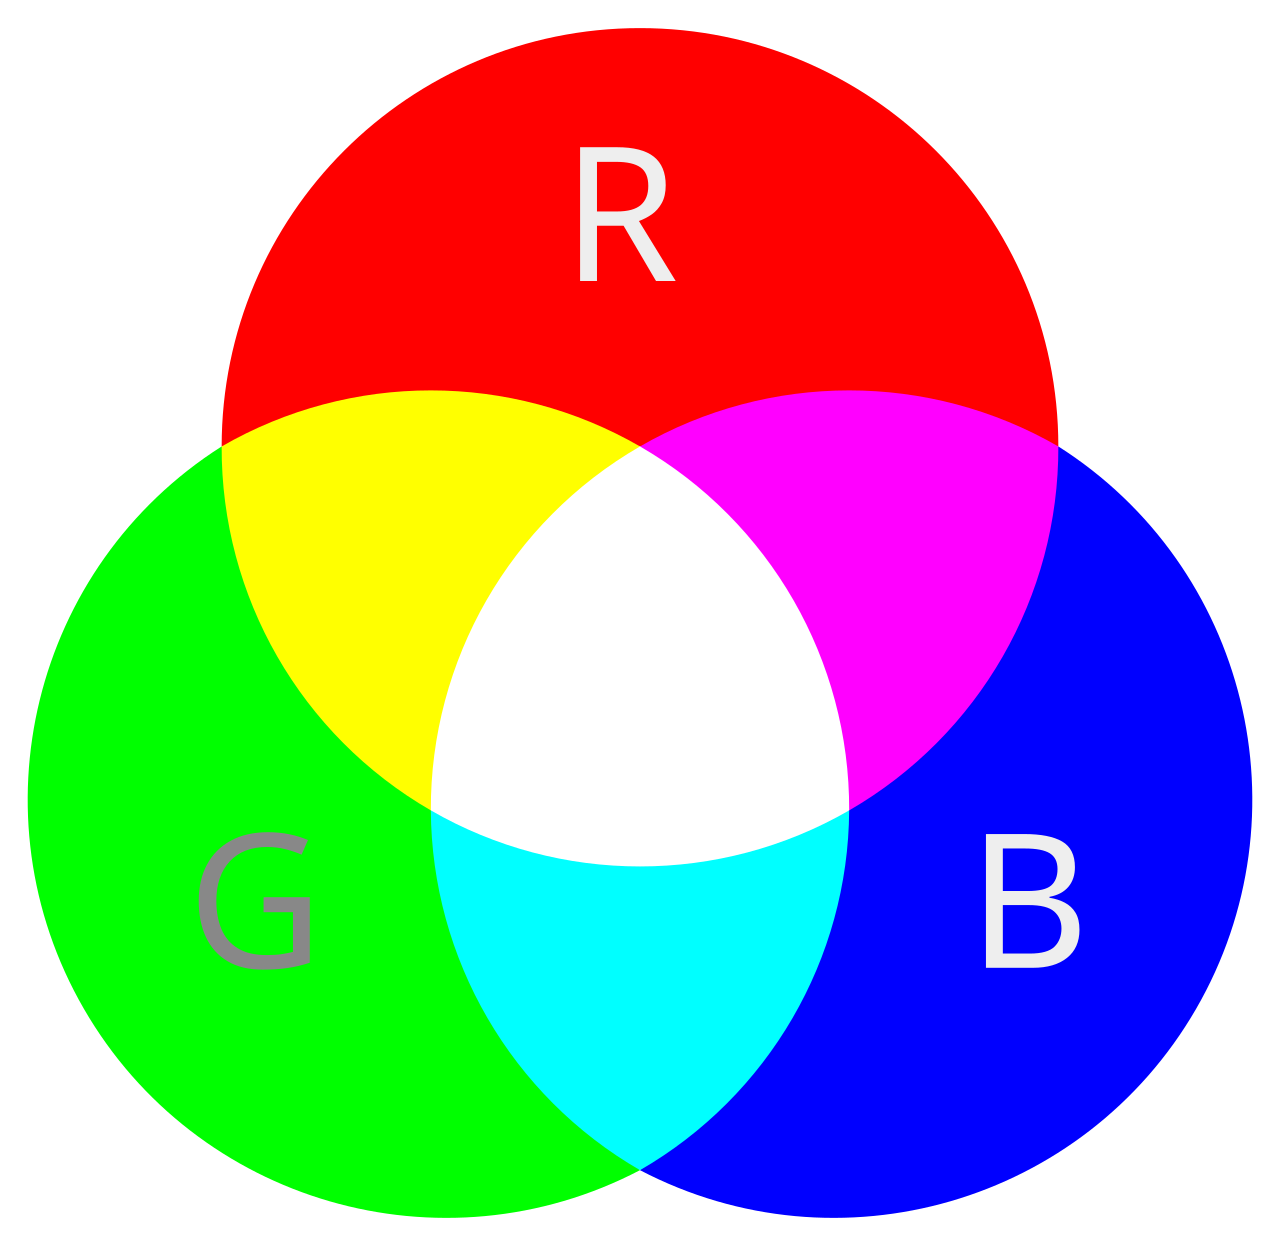
\includegraphics[height=4cm]{figs/rgb1.png}
     \caption{Vennův diagram pro RGB.}
   \end{subfigure}
   \begin{subfigure}{.4\textwidth}
     \centering
     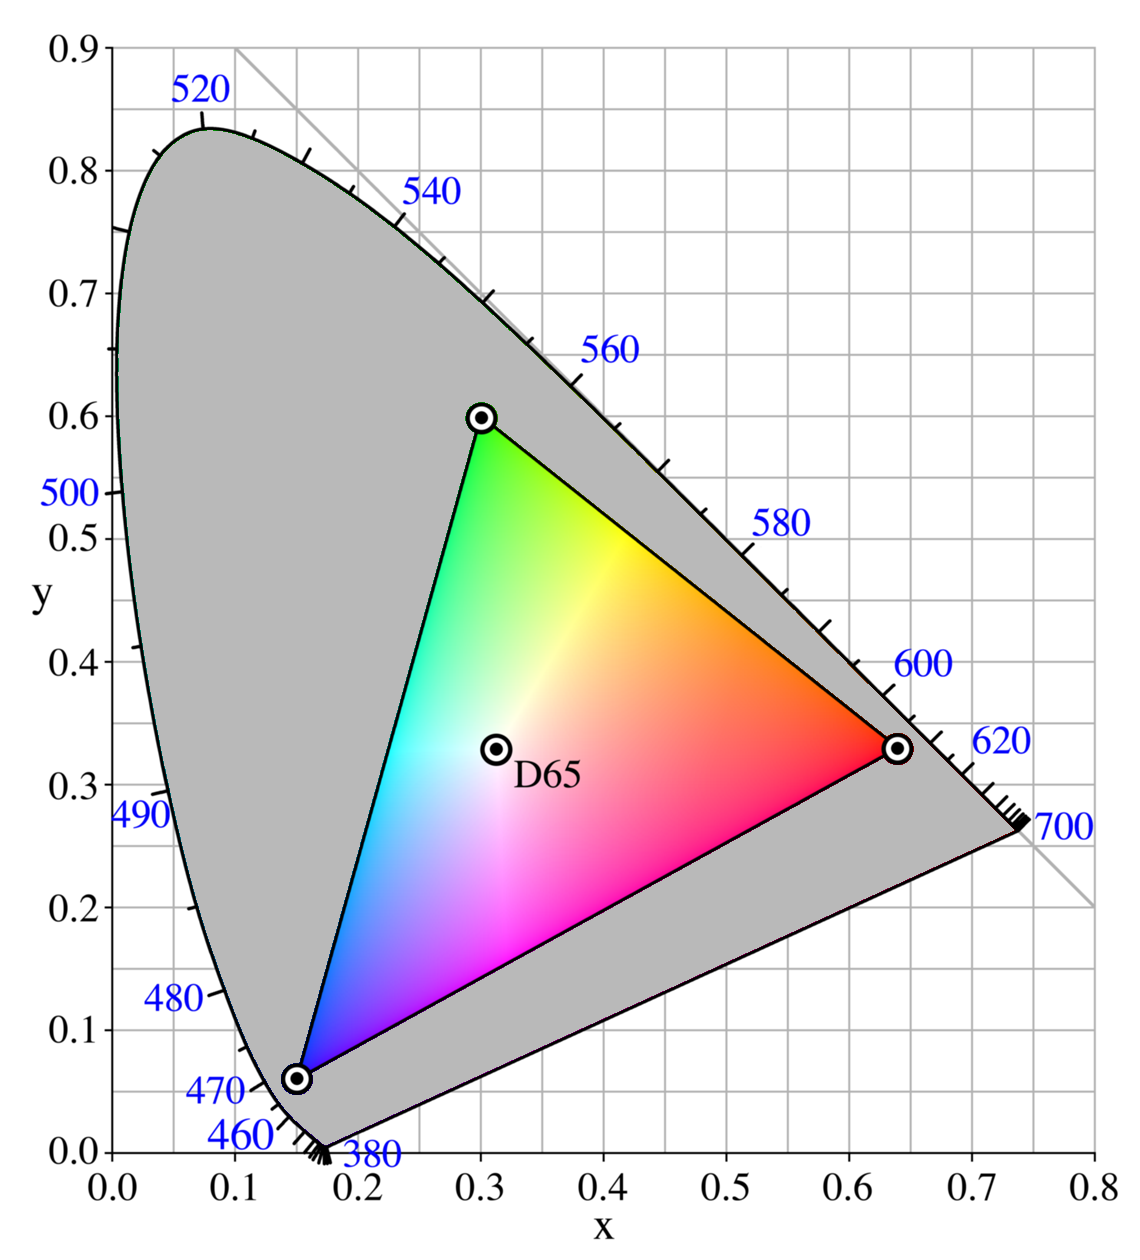
\includegraphics[height=4cm]{figs/rgb2.png}
     \caption{Pokrytí sRGB v chromatickém prostoru.}
   \end{subfigure}
  \end{figure}
  \end{itemize}
\end{frame}

\begin{frame}
  \frametitle{Jak funguje CMYK}
  \begin{itemize}[label=\textbullet]
   \item V podstatě úplně stejně jako RGB, akorát je \alert{subtraktivní}, takže
     slévání barev \alert{snižuje} jejich \uv{bělost}.
   \pause
   \item Jeho smyslem je representace barev pro tištění. Slevání v CMYK hrubě
     odpovídá slévání kapek inkoustu.
  \end{itemize}
  \pause
  \begin{figure}[H]
    \vspace*{-1em}
   \centering
   \begin{subfigure}{.4\textwidth}
     \centering
     
\includegraphics[height=4cm]{figs/cmyk1.png}
     \caption{Vennův diagram pro CMYK.}
   \end{subfigure}
   \begin{subfigure}{.55\textwidth}
     \centering
     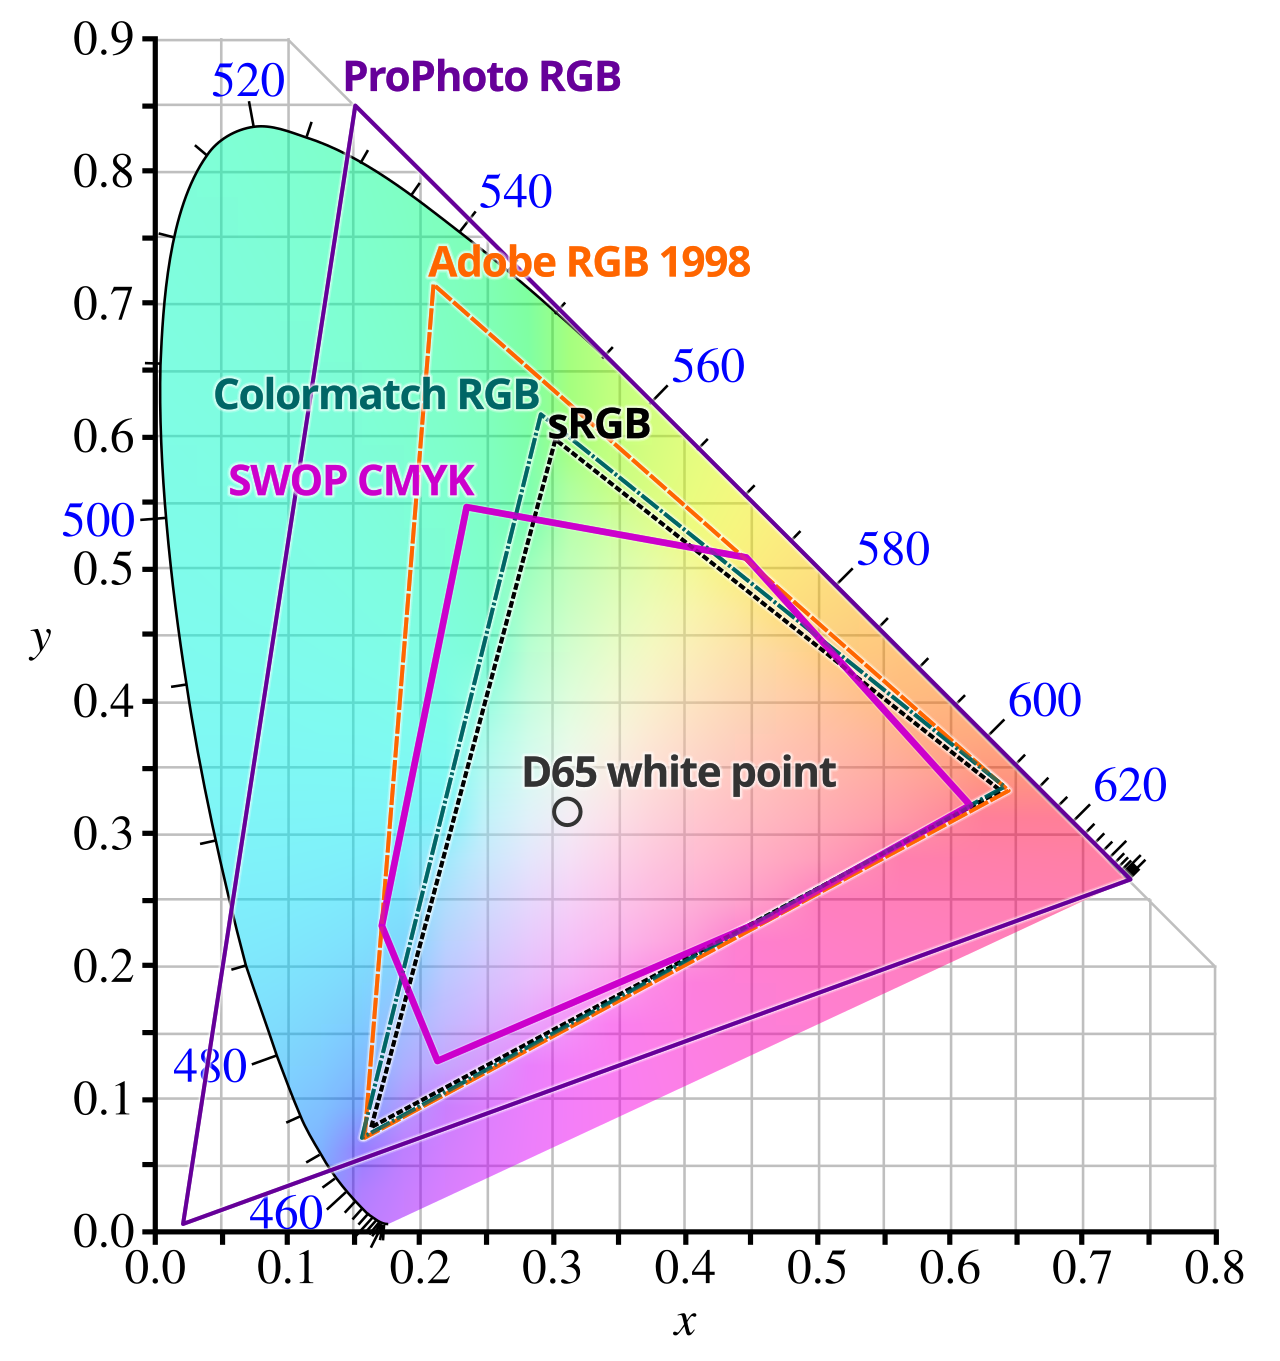
\includegraphics[height=4cm]{figs/cmyk2.png}
     \caption{Srovnání CMYK a typů RGB v chromatickém prostoru.}
   \end{subfigure}
  \end{figure}
\end{frame}

\begin{frame}
  \frametitle{Jak fungují HSL a HSV}
  \begin{itemize}[label=\textbullet]
    \item Zkratka \alert{HSL}, resp. \alert{HSV}, stojí za hue -- saturation --
      lightness, resp. hue -- saturation -- value.
    \pause
  \item Jsou to \uv{válcové} geometrie barev na rozdíl od RGB a CMYK, které jsou
    \uv{krychlové}:
  \pause
  \begin{itemize}[label=$\circ$]
    \item \alert{hue} je úhel (pozice barvy na obvodu válce),
    \item \alert{saturation} je vzdálenost od středu,
    \item \alert{value/lightness} je výška.
  \end{itemize}
  \pause
  \item Aditivní primární a sekundární barvy (červená, žlutá, zelená, cyanová,
    modrá, magenta) a kombinace libovolných dvou po sobě jdoucích (tzv.
    \uv{čisté} barvy) jsou umístěny podél obvodu válce se saturation $1$ a
    lightness $0.5$ (nebo value $1$). 
  \end{itemize}
\end{frame}

\begin{frame}
  \frametitle{Jak fungují HSL a HSV}
  \begin{figure}[H]
   \centering
   \begin{subfigure}{.45\textwidth}
     \centering
     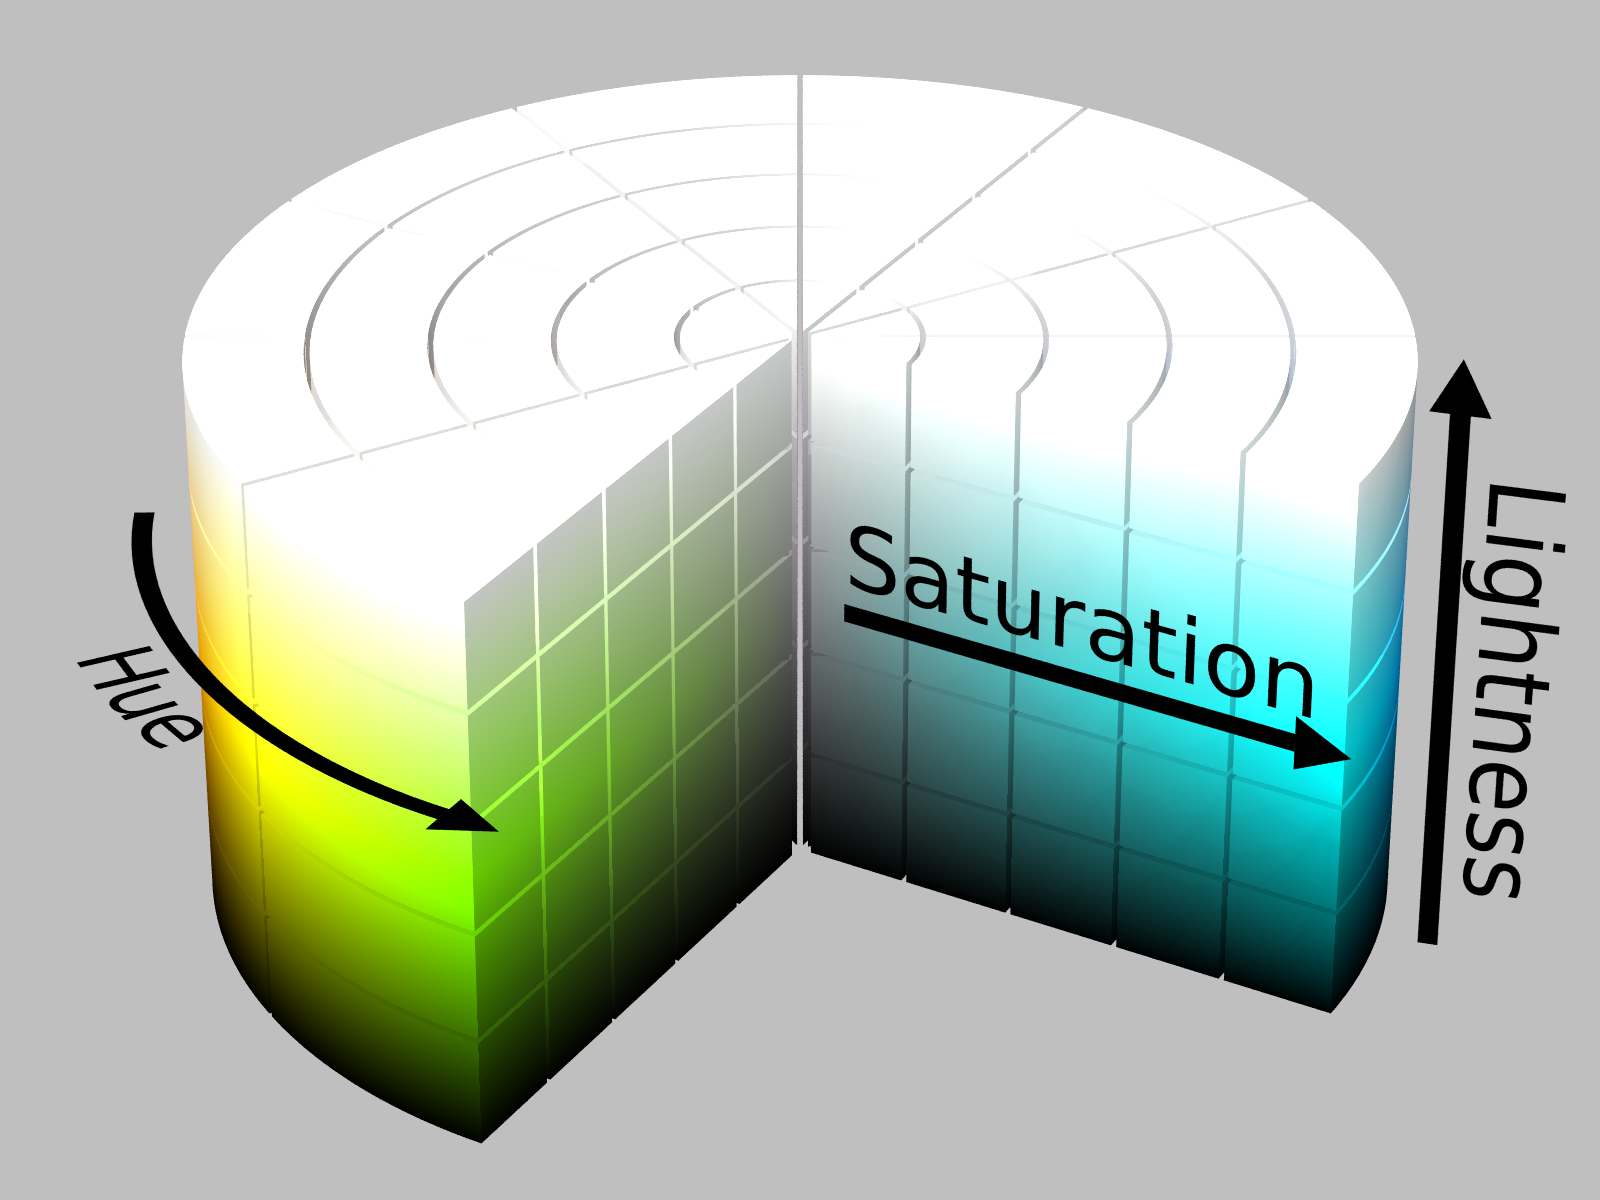
\includegraphics[height=3cm]{figs/hsl1.png}
     \caption{Válec HSL.}
   \end{subfigure}
   \begin{subfigure}{.45\textwidth}
     \centering
     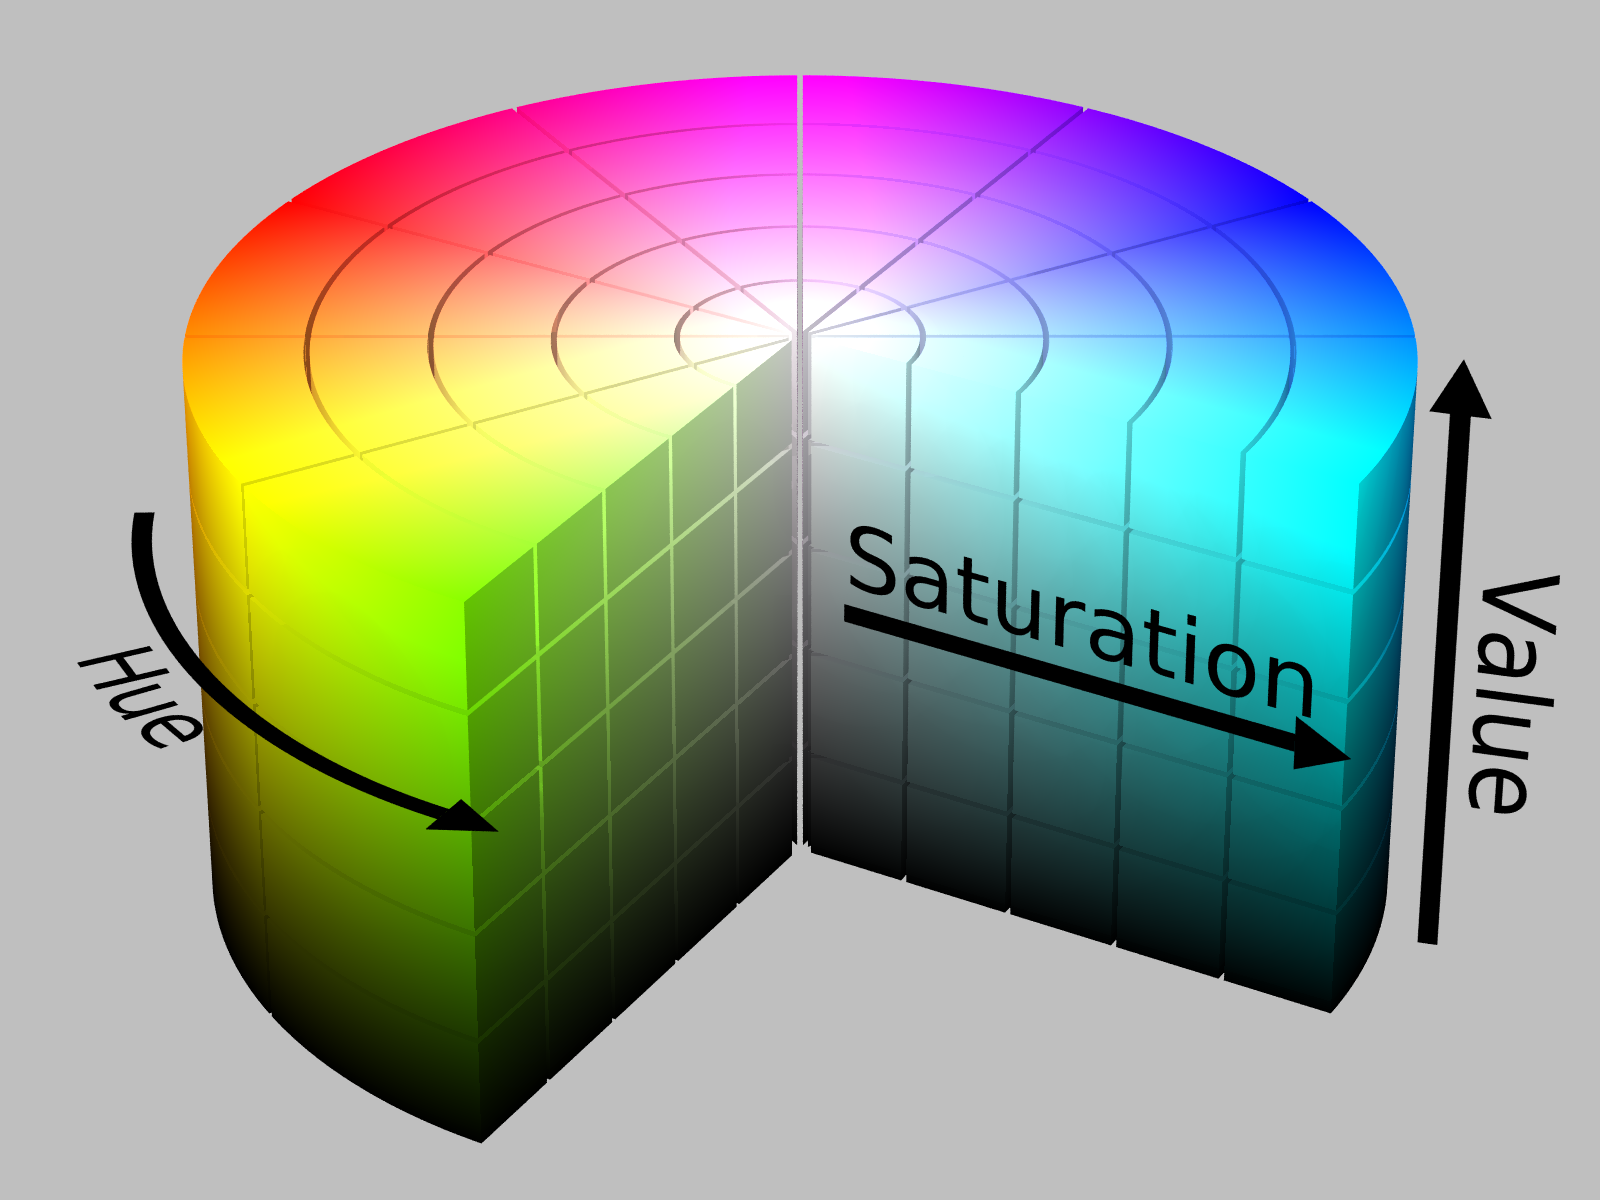
\includegraphics[height=3cm]{figs/hsl2.png}
     \caption{Válec HSV.}
   \end{subfigure}
   \begin{subfigure}{.45\textwidth}
     \vspace*{-2em}
     \centering
     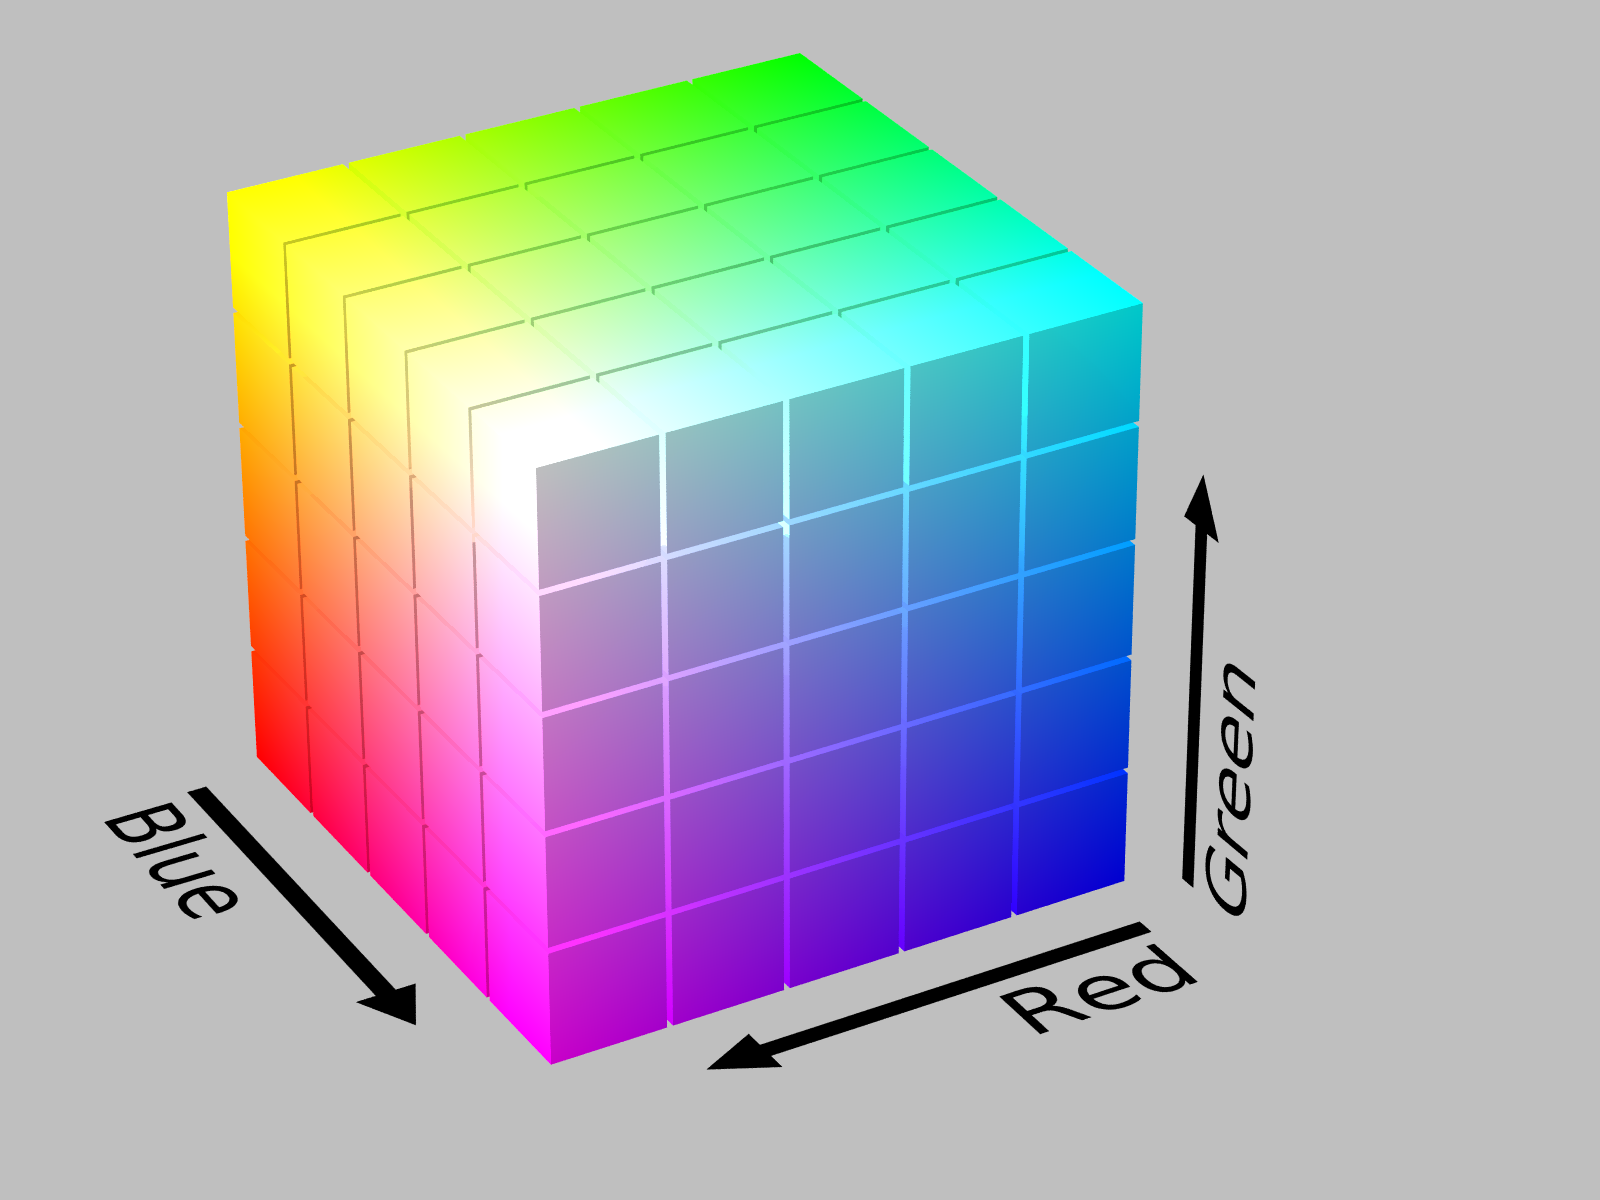
\includegraphics[height=3cm]{figs/hsl3.png}
     \caption{Krychle RGB.}
   \end{subfigure}
  \end{figure}
\end{frame}

\begin{frame}
  \frametitle{Jak funguje OKLCH}
  \begin{itemize}[label=\textbullet]
    \item Smyslem OKLCH (L -- lightness, c -- chroma, h -- hue) je zachovat
      klady HSL a HSV representací, ale vylepšit \uv{plynulost} přechodu mezi
      barvami.
    \pause
    \item Jde rovněž o válcový model, který ale není rovnoměrný (v každé výšce a
      úhlu má různý poloměr).
  \end{itemize}
  \pause
  \begin{figure}[H]
   \centering
   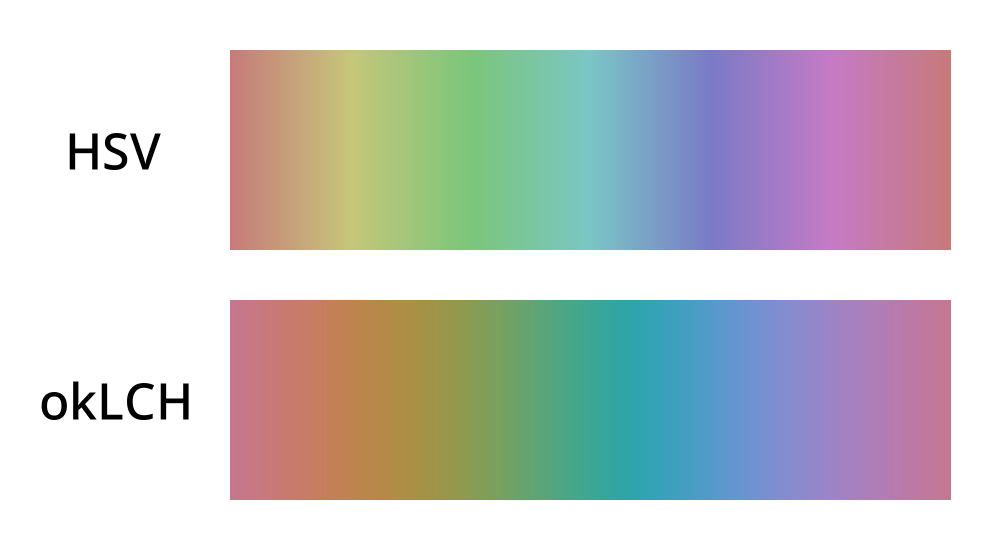
\includegraphics[height=3cm]{figs/oklch1.png}
   \caption*{Srovnání HSV a OKLCH.}
  \end{figure}
\end{frame}

\begin{frame}
  \frametitle{Jak funguje OKLCH}
  \begin{figure}[H]
   \centering
   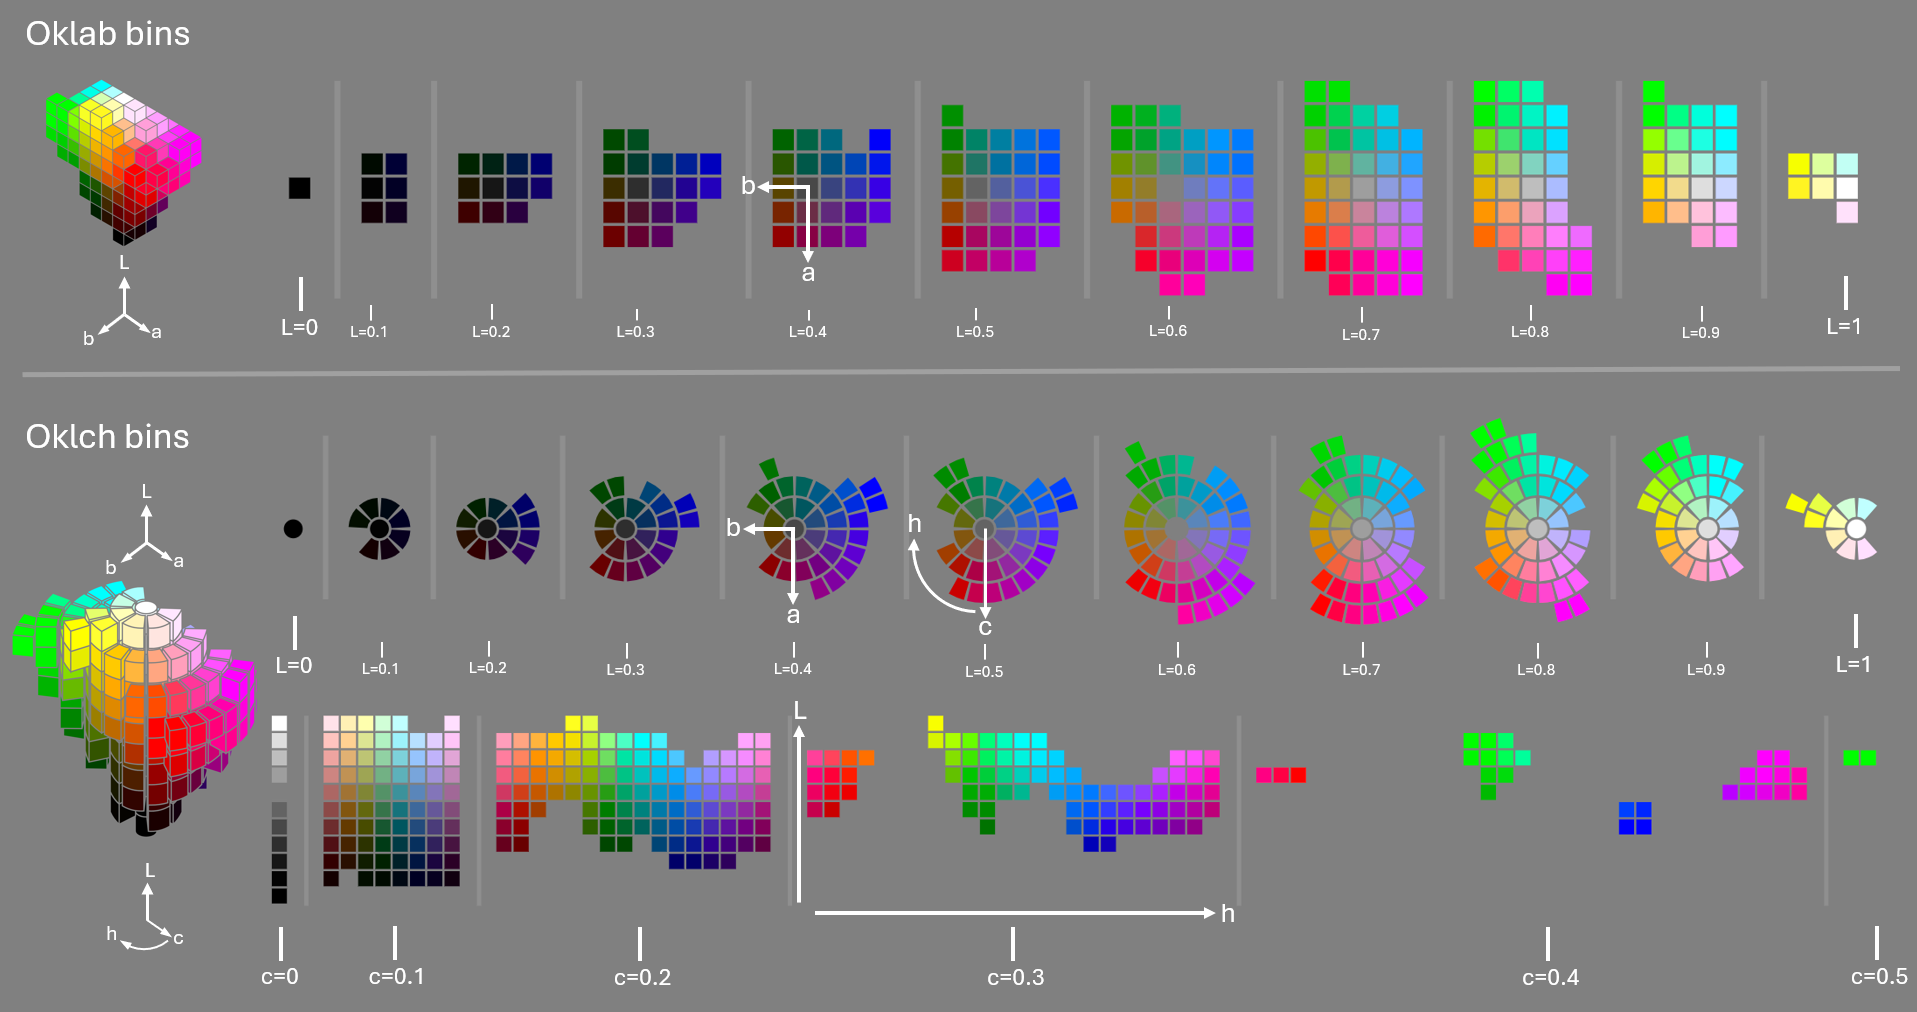
\includegraphics[height=6cm]{figs/oklch2.png}
   \caption*{Průřez OKLCH válcem.}
  \end{figure}
\end{frame}

\begin{frame}
  \frametitle{Jak funguje YUV}
  \begin{itemize}[label=\textbullet]
   \item Původním smyslem modelu bylo zobrazení barev na starých televizích.
   \pause
  \item Model odděluje barevnou informaci (osy U a V) od světelné informace (osa
    Y) podobně jako HSL.
  \pause
  \item To umožňovalo posílat informaci o světlosti barvy odděleně, takže
    černobílé televizory nemusely přijímat úplný signál.
  \pause
  \item Dnes má model stále omezené využití při kompresi, neboť lze světelné i
    barevné informaci určit hloubku (počet bitů) nezávisle s lineární ztrátou
    informace.
  \pause
  \item Tím je model výhodnější pro kompresi než třeba HSL, kde snížení hloubky
    saturation sníží množství representovatelných barev kvadraticky.
  \end{itemize}
\end{frame}

\begin{frame}
  \frametitle{Jak funguje YUV}
  \begin{figure}[H]
   \centering
   \begin{subfigure}{.4\textwidth}
     \centering
     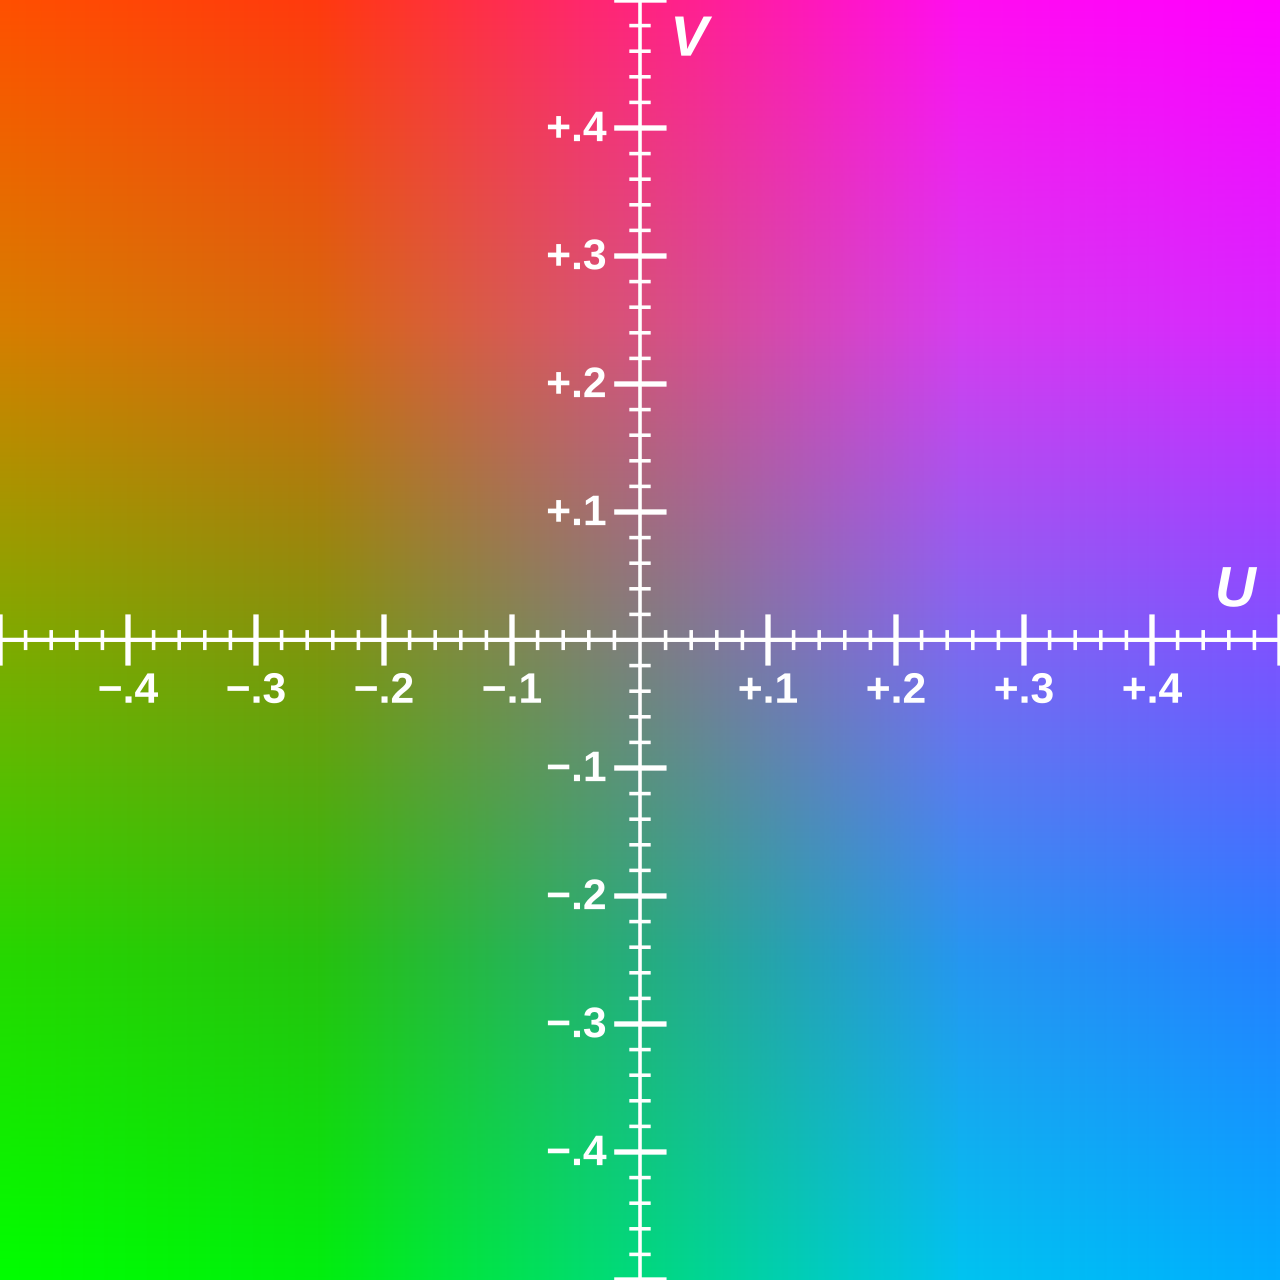
\includegraphics[height=5cm]{figs/yuv1.png}
     \caption{Rovina $UV$ s $Y = 0.5$.}
   \end{subfigure}
   \begin{subfigure}{.55\textwidth}
     \centering
     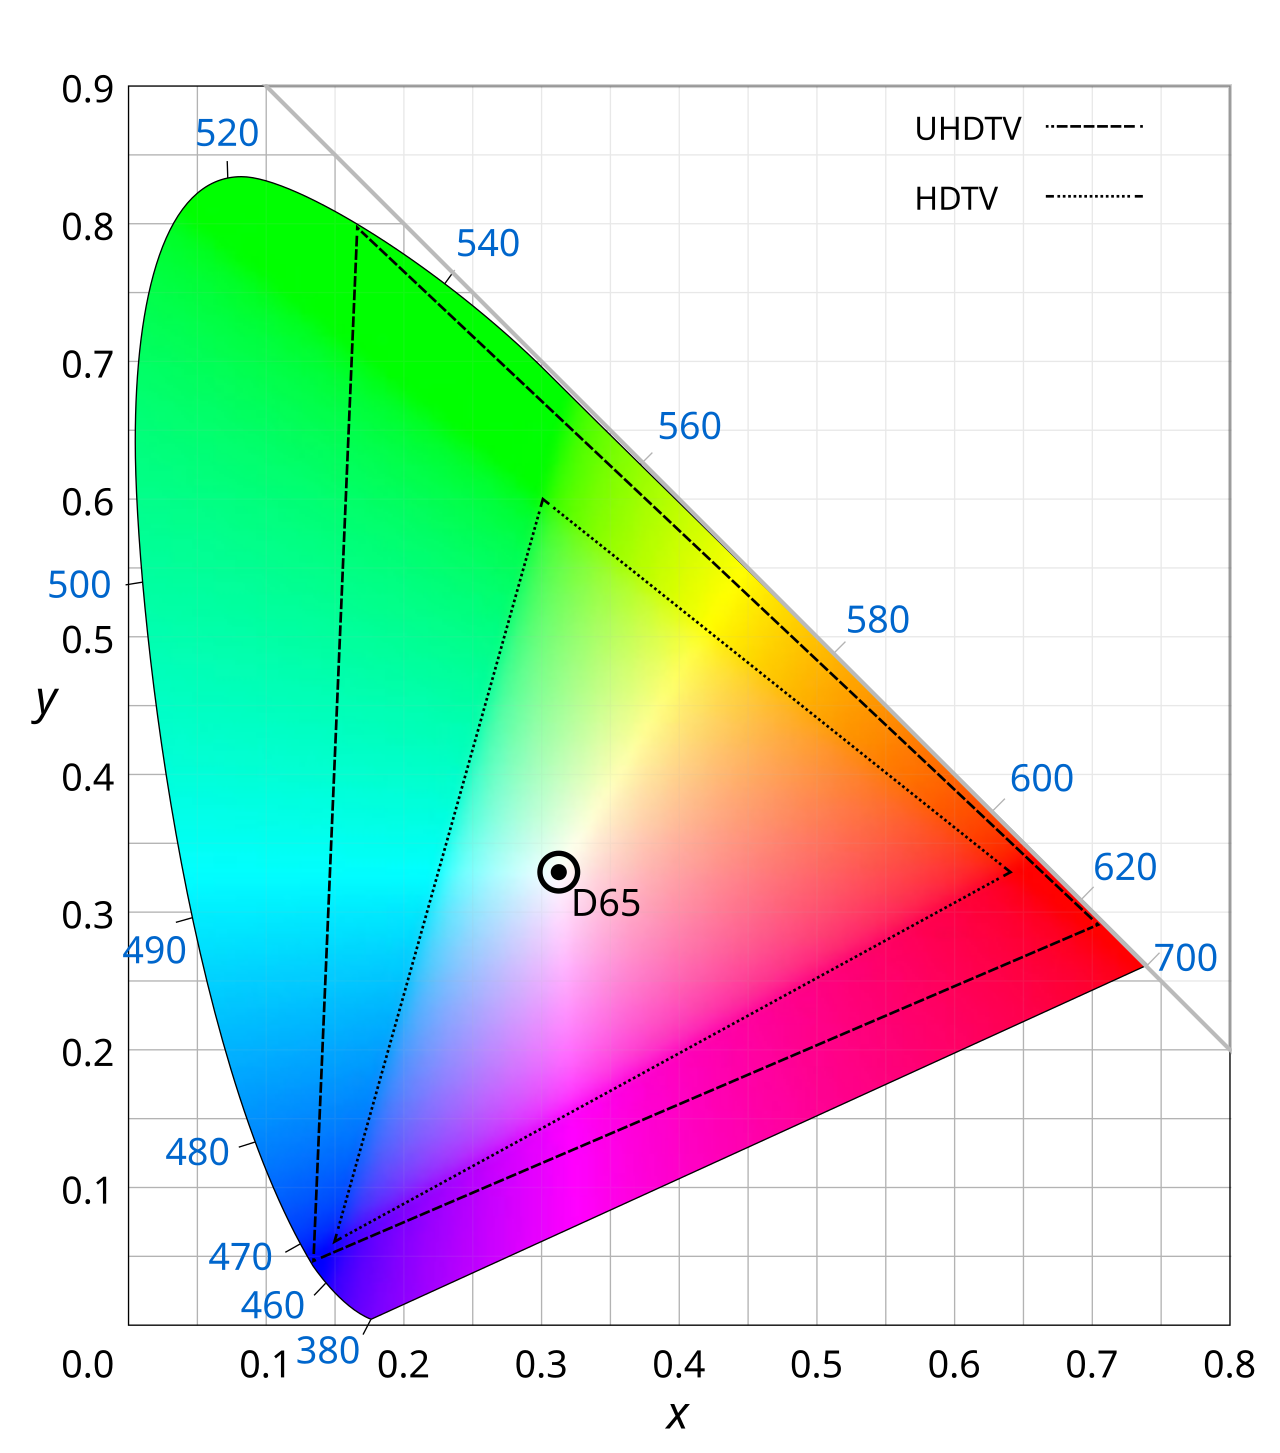
\includegraphics[height=5cm]{figs/yuv2.png}
     \caption{Pokrytí HDTV a UHDTV v chromatickém prostoru.}
   \end{subfigure}
  \end{figure}
\end{frame}

\end{document}
